\documentclass[11pt]{article}
\usepackage{enumitem}
\usepackage{listings}
\usepackage[listings]{tcolorbox}
\usepackage{tikz}
\usepackage{url}
\usepackage{alltt}

%\usepackage{algorithm2e}
\usetikzlibrary{arrows,automata,shapes}
\tikzstyle{block} = [rectangle, draw, fill=blue!20, 
    text width=5em, text centered, rounded corners, minimum height=2em]
\tikzstyle{bt} = [rectangle, draw, fill=blue!20, 
    text width=4em, text centered, rounded corners, minimum height=2em]

\lstset{ %
language=Java,
basicstyle=\ttfamily,commentstyle=\scriptsize\itshape,showstringspaces=false,breaklines=true,numbers=left}
\newtcbinputlisting{\codelisting}[3][]{
    extrude left by=1em,
    extrude right by=2em,
    listing file={#3},
    fonttitle=\bfseries,
    listing options={basicstyle=\ttfamily\footnotesize,numbers=left,language=Java,#1},
    listing only,
    hbox,
}
\lstdefinelanguage{JavaScript}{
  keywords={typeof, new, true, false, catch, function, return, null, catch, switch, var, if, in, while, 
do, else, case, break},
  keywordstyle=\color{blue}\bfseries,
  ndkeywords={class, export, boolean, throw, implements, import, this},
  ndkeywordstyle=\color{darkgray}\bfseries,
  identifierstyle=\color{black},
  sensitive=false,
  comment=[l]{//},
  morecomment=[s]{/*}{*/},
  commentstyle=\color{purple}\ttfamily,
  stringstyle=\color{red}\ttfamily,
  morestring=[b]',
  morestring=[b]''
}


\newtheorem{defn}{Definition}
\newtheorem{crit}{Criterion}

\newcommand{\handout}[5]{
  \noindent
  \begin{center}
  \framebox{
    \vbox{
      \hbox to 5.78in { {\bf Software Testing, Quality Assurance and Maintenance } \hfill #2 }
      \vspace{4mm}
      \hbox to 5.78in { {\Large \hfill #5  \hfill} }
      \vspace{2mm}
      \hbox to 5.78in { {\em #3 \hfill #4} }
    }
  }
  \end{center}
  \vspace*{4mm}
}

\newcommand{\lecture}[4]{\handout{#1}{#2}{#3}{#4}{Lecture #1}}
\topmargin 0pt
\advance \topmargin by -\headheight
\advance \topmargin by -\headsep
\textheight 8.9in
\oddsidemargin 0pt
\evensidemargin \oddsidemargin
\marginparwidth 0.5in
\textwidth 6.5in

\parindent 0in
\parskip 1.5ex
%\renewcommand{\baselinestretch}{1.25}

\begin{document}

\lecture{4 --- January 15, 2025}{Winter 2025}{Patrick Lam}{version 1}

Before we continue with operational semantics, I'm going to talk about
mutation analysis.

Remember, we have this problem: when do we stop testing? How do we
know that our test suite is good enough?

We talked about coverage, but we also saw how it's far from perfect.

\section*{Mutation Analysis}
What if we checked whether our test suite can detect changes to the program?
If it can, then it is detecting something, at least.

A \emph{mutant} is a version of the program that has been somehow modified
(in one place, usually an operator or identifier switch.)

Remember that tests contain three phases: arrange, act, assert.
Running on a modified program, the test suite might trigger errors
during the ``act'' phase. Or, it can detect where the program is
giving a different output during the ``assert'' phase.

Another way of looking at this is that we are fuzzing the test suite
(by modifying the program) and checking that the test suite is doing what it
should (that is, finding broken programs).

\paragraph{Example} Here's a program and some mutants. We can use the language grammar
to create the mutants.

{
  \small
\begin{minipage}[t]{.5\textwidth}
\begin{alltt}
// original
int min(int a, int b) \{
  int minVal;
  minVal = a;

  if (b < a) \{


    minVal = b;



  \}
  return minVal;
\}
\end{alltt}
\end{minipage} \begin{minipage}[t]{.5\textwidth}
\begin{alltt}
// with mutants
int min(int a, int b) \{
  int minVal;
  minVal = a;
  minVal = b;               // \(\Delta 1\)
  if (b < a) \{
  if (b > a) \{              // \(\Delta 2\)
  if (b < minVal) \{         // \(\Delta 3 \)
    minVal = b;
    BOMB();                 // \(\Delta 4\)
    minVal = a;             // \(\Delta 5\)
    minVal = failOnZero(b); // \(\Delta 6\)
  \}
  return minVal;
\}
\end{alltt}
\end{minipage}
}

Conceptually we've shown 6 programs, but we display them together for 
convenience. You'll find code in {\tt code/L04/minval.c} in the {\tt pdfs} repo.

We're generating mutants $m$ for the original program $m_0$.
\begin{defn}
Test case $t$ \emph{kills} $m$ if running $t$ on $m$ gives different 
output than running $t$ on $m_0$.
\end{defn}

We use these mutants to evaluate test suites. Here's a simple test suite. I'm abstractly representing a JUnit test case
by a tuple; assume that it calls {\tt min()} and asserts on the return value. You can fill out this table.

\begin{center}
\begin{tabular}{lcccccc}
  & $\Delta$ 1 & $\Delta$ 2 & $\Delta$ 3 & $\Delta$ 4 & $\Delta$ 5 & $\Delta$ 6\\ 
  $\langle a = 0, b = 1, \mathrm{exp} = 0 \rangle$   & kill & & -- \\
  $\langle a = 1, b = 0, \mathrm{exp} = 0 \rangle$   & --   & & -- \\
  $\langle a = 1, b = 1, \mathrm{exp} = 1 \rangle$   &      & & -- \\
  $\langle a = 1, b = 349, \mathrm{exp} = 1 \rangle$ &      & & -- \\
\end{tabular}
\end{center}

Note that, for instance, $\Delta$ 3 is not killable; if you look at the modification,
you can see that it is equivalent to the original.

The idea is to use mutation analysis to evaluate test suite quality/improve test suites.
Good test suites ought to be effective at killing mutants.

\subsection*{General Concepts}

Mutation analysis relies on two hypotheses, summarized from \cite{delgado-perez18:_evaluat_mutat_testin_nuclear_indus_case_study}.

The \emph{Competent Programmer Hypothesis} posits that programmers usually are almost right.
There may be ``subtle, low-level faults''. Mutation analysis introduces faults that
are similar to such faults. (We can think of exceptions to this hypothesis---if
the code isn't tested, for instance; or, if the code was written to the wrong
requirements.)

The \emph{Coupling Effect Hypothesis} posits that complex faults are the result of
simple faults combining; hence, detecting all simple faults will detect many
complex faults.

If we accept these hypotheses, then test suites that are good at ensuring program
quality are also good at killing mutants.

Mutation is hard to apply by hand, and automation is
complicated.  The testing community generally considers mutation to be
a ``gold standard'' that serves as a benchmark against which to
compare other testing criteria against. For example, consider a test suite
$T$ which ensures statement coverage. What can mutation analysis say about
how good $T$ is?

Mutation analysis proceeds as follows.

\begin{enumerate}[noitemsep]
\item \emph{Generate mutants:} apply mutation operators to the program to get a set of mutants $M$. 
\item \emph{Execute mutants:} execute the test suite on each mutant and collect suite pass/fail results.
\item \emph{Classify:} interpret the results as either killing each mutant or not; a failed test suite execution implies a killed mutant.
\end{enumerate}

Although you could generate mutants by hand, typically you would tend to use a tool which parses the input program, applies a mutation operator, and then unparses back to source code, which is then recompiled.

Executing the mutants can be computationally expensive, since you have to run the entire test suite on each of the mutants. This is a good time to use all the compute infrastructure available to you.

Generating and executing are computationally expensive, but classifying is worse, because it requires manual analysis. In particular, a not-killed result could be due to an equivalent mutant (like $\Delta$ 3 above); compilers can help, but the problem is fundamentally undecidable. Alternately, not-killed could be because the test suite isn't good enough. It's up to you to distinguish these cases. On the next page, ``bogus mutants'' denotes equivalent, stillborn and trivial mutants.

You would normally want to then craft new test cases to kill the non-equivalent mutants that you found.
\subsection*{Testing Programs with Mutation}
Here's a picture that illustrates a variant of the above workflow.

\begin{center}
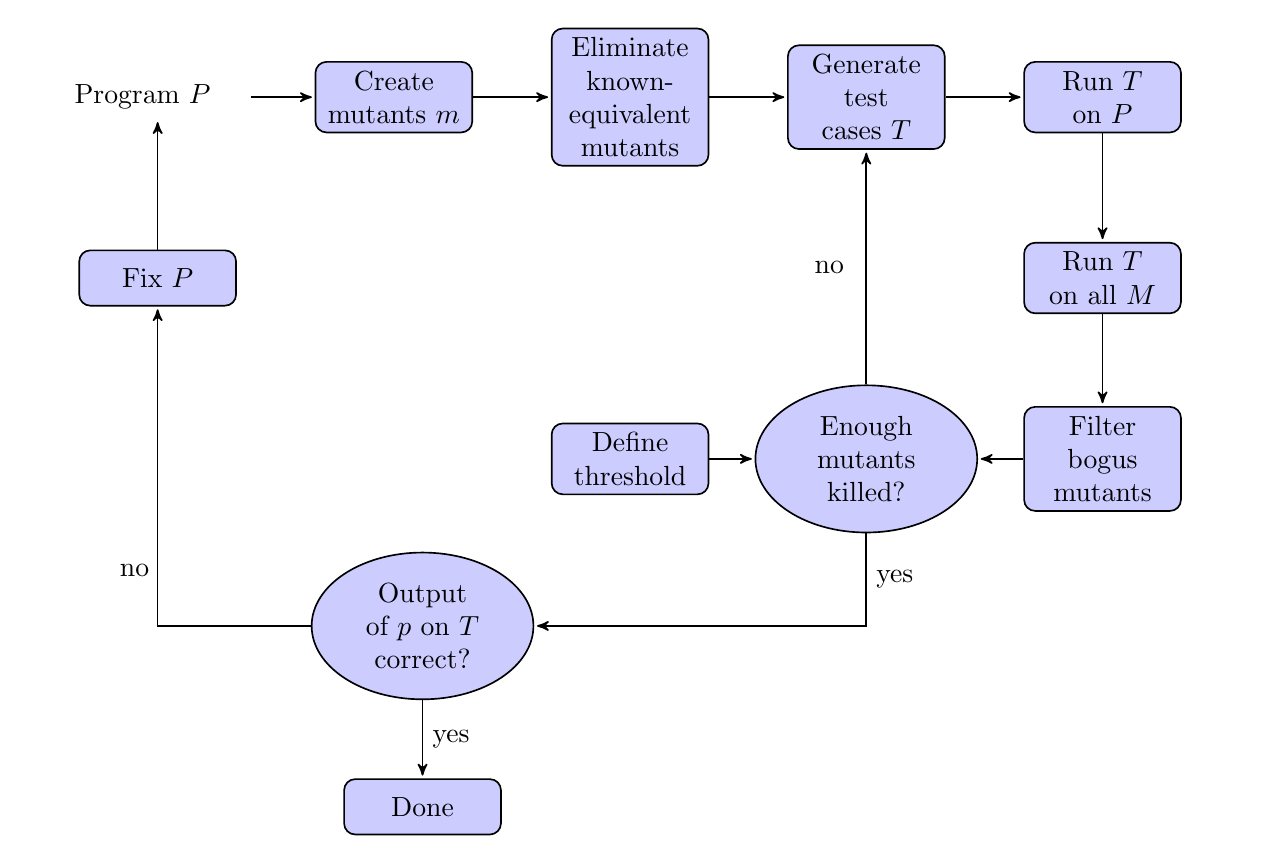
\begin{tikzpicture}[->,>=stealth',shorten >=1pt,auto,node distance=3cm,
                    text width=4em,
                    semithick,initial text=]
  \node[text width=6em] (p) {Program $P$};
  \node[block,right of=p] (create) {Create mutants $m$};
  \node[block,right of=create] (elim) {Eliminate known-equivalent mutants};
  \node[block,right of=elim] (gen) {Generate test cases $T$};
  \node[block,right of=gen] (runTonP) {Run $T$ on $P$};
  \node[block,below of=runTonP,yshift=2em] (runTonM) {Run $T$ on all $M$};
  \node[block, below of=runTonM,yshift=2em] (filter) {Filter bogus mutants};
  \node[shape=ellipse, text centered, fill=blue!20, draw, text width=5em, left of=filter] (enough) {Enough mutants killed?};
  \node[block, left of=enough] (findThreshold) {Define threshold};
  \node[shape=ellipse, text centered, fill=blue!20, draw, text width=5em, below left of=enough,xshift=-10em] (correct) {Output of $p$ on $T$ correct?};
  \node[block, below of=correct,yshift=2em] (done) {Done};
  \node[block, below of=p,yshift=2em] (fixP) {Fix $P$};

  \path (p) edge node {} (create)
        (create) edge node {} (elim)
        (elim) edge node {} (gen)
        (gen) edge node {} (runTonP)
        (runTonP) edge node {} (runTonM)
        (runTonM) edge node {} (filter)
        (filter) edge node {} (enough)
        (findThreshold) edge node {} (enough)
        (correct) edge node {yes} (done)
        (fixP) edge node {} (p);
  \draw (correct) -| node[xshift=3em,yshift=2em] {no} (fixP); % no
  \draw (enough.north) -- node[xshift=2.5em] {no} (gen);
  \draw (enough) |- node[near start] {yes} (correct);
\end{tikzpicture}
\end{center}

\subsection*{Generating Mutants}

Now let's see how to generate mutants; this is similar to
grammar-based fuzzing (but of the code).  For mutation analysis,
strings will always be programs.

\begin{defn}
Ground string: a (valid) string belonging to the language of the grammar (i.e. 
a programming language grammar).
\end{defn}

\begin{defn}
Mutation Operator: a rule that specifies syntactic variations of
strings generated from a grammar.
\end{defn}

\begin{defn}
Mutant: the result of one application of a mutation operator to a 
ground string.
\end{defn}

The workflow is to parse the ground string (original program), apply a
mutation operator, and then unparse.

It is generally difficult to find good mutation operators. One example
of a bad mutation operator might be to change all boolean expressions to
``true''. Fortunately, the research shows that you don't need many
mutation operators---the right 5 will do fine.

Some points:
\begin{itemize}[noitemsep]
\item How many mutation operators should you apply to get mutants? \emph{One.}
\item Should you apply every mutation operator everywhere it might apply? \emph{Too much work; choose randomly.}
\end{itemize}

\paragraph{Killing Mutants.} 
We can also define a mutation score, which is the percentage of mutants killed.

To use mutation analysis for generating test cases, one would measure
the effectiveness of a test suite (the mutation score), and keep adding
tests until reaching a desired mutation score.

So far we've talked about requiring differences in the \emph{output}
for mutants.  We call such mutants {\bf strong mutants}.  We can relax
this by only requiring changes in the \emph{state}, which we'll call
{\bf weak mutants}.

In other words, 
\begin{itemize}[noitemsep]
\item \emph{strong mutation}: fault must be \emph{reachable},
\emph{infect} state, and \emph{\bf propagate} to output.
\item \emph{weak mutation}: a fault which kills a mutant need only be
\emph{reachable} and \emph{infect state}.
\end{itemize}
Supposedly, experiments show that weak and strong mutation require
almost the same number of tests to satisfy them.

Let's consider mutant $\Delta 1$ from above, i.e. we change
{\tt minVal = a} to {\tt minVal = b}. In this case:
\begin{itemize}[noitemsep]
\item reachability: unavoidable;
\item infection: need $b \neq a$;
\item propagation: wrong {\tt minVal} needs to return to the caller;
that is, we can't execute the body of the {\tt if} statement, so we
need $b > a$.
\end{itemize}
A test case for strong mutation is therefore $a = 5, b = 7$ (return
value = \textvisiblespace, expected \textvisiblespace), and for
weak mutation $a = 7, b = 5$ (return value = \textvisiblespace, expected
\textvisiblespace).

Now consider mutant $\Delta 3$, which replaces {\tt b < a} with {\tt 
b < minVal}. This mutant is an equivalent mutant, since {\tt a = minVal}.
(The infection condition boils down to ``false''.)

Equivalence testing is, in its full generality, undecidable, but we can always
estimate.

\paragraph{Another example.} Given the ground string {\tt x = a + b},
we might create mutants {\tt x = a - b}, {\tt x = a * b}, etc.
A possible original on the
left and a mutant on the right:

\begin{minipage}{.5\textwidth} 
\begin{alltt}
int foo(int x, int y) \{ // original
  if (x > 5) return x + y;
  else return x;
\}
\end{alltt}
\end{minipage}\begin{minipage}{.5\textwidth}
\begin{alltt}
int foo(int x, int y) \{ // mutant
  if (x > 5) return x - y;
  else return x;
\}
\end{alltt}
\end{minipage}
~\\[3em]
In this example, the test case $\langle 6, 2 \rangle$ will kill
 the mutant, since it returns 8 for the original and 4 for the mutant,
while the case $\langle 6, 0 \rangle$ will not kill the mutant,
since it returns 6 in both cases.

Once we find a test case that kills a mutant, we can forget the
mutant and keep the test case. The mutant is then \emph{dead}.

The other thing that can happen when you are running a test case on a mutant is
that it loops indefinitely. You'd want to use a timeout when running testcases,
and then you have a timeout failure, which you can presumably use to distinguish
the mutant from the original.

\paragraph{Uninteresting Mutants.} Three kinds of mutants are uninteresting:
\begin{itemize}[noitemsep]
\item \emph{stillborn}: such mutants cannot compile (or immediately crash);
\item \emph{trivial}: killed by almost any test case;
\item \emph{equivalent}: indistinguishable from original program.
\end{itemize}

The usual application of program-based mutation is to individual statements
in unit-level (per-method) testing.

\section*{Implementing Mutation Analysis}
Recall that the goals of mutation analysis are to evaluate test suites by:
\begin{enumerate}[noitemsep]
\item mimicking (and hence testing for) typical mistakes;
\item encoding knowledge about specific kinds of effective tests in practice, e.g.
statement coverage ($\Delta 4$), checking for 0 values ($\Delta 6$).
\end{enumerate}

We'll see a number of mutation operators, although precise
definitions are specific to a language of interest. Typical mutation
operators will encode typical programmer mistakes, e.g. by changing
relational operators or variable references; or common testing heuristics, 
e.g. fail on zero. Some mutation operators are better than others.

One tool you can use for mutation analysis is PIT.  It mutates your
program, reruns your test suite, tells you how it went. You need to
distinguish equivalent vs. not-killed.  You can find a more exhaustive
list of mutation operators in the PIT documentation:

\begin{center}
\url{https://pitest.org/quickstart/mutators/}
\end{center}

How
many mutation operators can you invent for the
following code?

{ \Large
\begin{lstlisting}
int mutationTest(int a, b) { 
  int x = 3 * a, y;
  if (m > n) {
    y = -n;
  }
  else if (!(a > -b)) {
    x = a * b;
  }
  return x;
}
\end{lstlisting}
}

[Absolute value insertion, operator replacement, scalar variable replacement,
  statement replacement with crash statements\ldots]

\paragraph{Exercise.} Come up with a test case to kill each of these types of
mutants.

\begin{itemize}
\item {\bf ABS}: Absolute Value Insertion\\
{\tt x = 3 * a}
$\Longrightarrow$ {\tt x = 3 * abs(a)}, {\tt x = 3 * -abs(a)}, {\tt x = 3 * failOnZero(a)};
\item {\bf ROR}: Relational Operator Replacement\\
{\tt if (m > n)} $\Longrightarrow$ {\tt if (m >= n)}, {\tt if (m < n)}, {\tt if (m <= n)}, {\tt if (m == n)}, {\tt if (m != n)}, {\tt if (false)}, {\tt if (true)}
\item {\bf UOD}: Unary Operator Deletion\\
{\tt if (!(a > -b))} $\Longrightarrow$ {\tt if (a > -b)}, {\tt if (!(a > b))}
\end{itemize}


\section*{Is Mutation Analysis Any Good?}
We've talked about mutation analysis as a metric for evaluating test
suites and making sure that test suites exercise the system under test
sufficiently. The problem with metrics is that they can be gamed, or
that they might measure not quite the right thing. When using metrics,
it's critical to keep in mind what the right thing is. In this case,
the right thing is the fault detection power of a test suite.

Researchers (including some at Waterloo) set out to determine just that. They carried out a
study, using realistic code, where they isolated a number of bugs, and
evaluated whether or not there exists a correlation between real fault
detection and mutant detection.

\paragraph{Summary.} The answer is {\bf yes}: test suites
that kill more mutants are also better at finding real bugs. The
researchers also investigated when mutation analysis fell short---they
enumerated types of bugs that mutation analysis, as currently
practiced, would not detect.

\paragraph{Methodology.} The authors used 5 open-source projects.
They isolated a total of 357 reproducible faults in these projects
using the projects' bug reporting systems and source control
repositories. They they generated 230,000 mutants using the
Major mutation framework and investigated the ability of
both developer-written test suites and automatically-generated
test suites (EvoSuite, Randoop, JCrasher) to detect the 357 faults.

For each fault, the authors started with a developer-written test
suite $T_{\mbox{\em \scriptsize bug}}$ that did not detect the fault. Then, using
the source repository, they extracted a developer-written test that
detects the fault. Call this suite $T_{\mbox{\em \scriptsize fix}}$. Does
$T_{\mbox{\em \scriptsize fix}}$ detect more mutants than $T_{\mbox{\em \scriptsize bug}}$?
If so, then we can conclude that the mutant behaves like a bug.

\paragraph{Results.} The authors found that Major-generated mutation
tests could detect 73\% of the faults.  In other words, for 73\% of
faults, some mutant will be killed by a test that also detects the
fault. Increasing mutation coverage thus also increases the likelihood
of finding faults.

The analogous numbers for branch coverage and statement coverage are,
respectively, 50\% and 40\%. Specifically: the 357 tests that find
faults only increase branch coverage 50\% of the time, and they only
increase statement coverage 40\% of the time. So: improving your test
suite often doesn't get rewarded with a better statement coverage
score, and half the time doesn't result in a better branch coverage
score. Conversely, improving statement coverage doesn't help find more bugs because
you're already reaching the fault, but you aren't sensitive to the erroneous state.

The authors also looked at the 27\% of remaining faults that
are not found by mutants. For 10\% of these, better mutation operators
could have helped. The remaining 17\% were not suitable for mutation analysis:
they were fixed by e.g. algorithmic improvements or code deletion.

\paragraph{Reference.}
Ren\'e Just, Darioush Jalali, Laura Inozemtseva, Michael D. Ernst,
Reid Holmes, and Gordon Fraser. ``Are Mutants a Valid Substitute for
Real Faults in Software Testing?''  In {\em Foundations of Software
Engineering} 2014. pp654--665.
\url{http://www.linozemtseva.com/research/2014/fse/mutant_validity/}

\section*{What Does (Graph) Coverage Buy You?}
We've talked about graph coverage, notably statement coverage (node
coverage) and branch coverage (edge coverage). They're popular because
they are easy to compute. But, are they any good? Reid Holmes (a
former Waterloo CS prof) and his then-PhD student Laura Inozemtseva set out to answer
that question.

\paragraph{Answer.} Coverage does not correlate with high quality
when it comes to test suites.
Specifically: test suites that are larger are better because
they are larger, not because they have higher coverage.

\paragraph{Methodology.} The authors picked 5 large programs
and created test suites for these programs by taking random
subsets of the developer-written test suites. They measured
coverage and they measured effectiveness (defined as \% mutants
detected; we've seen that detecting mutants is good, above).

\paragraph{Result.} In more technical terms: after controlling
for suite size, coverage is not strongly correlated with effectiveness.

Furthermore, stronger coverage (e.g. branch vs statement, logic vs branch)
doesn't buy you better test suites.

\paragraph{Discussion.} So why are we making you learn about
coverage? Well, it's what's out there, so you should know about it.
But be aware of its limitations.

Plus: if you are not covering some program element, then you obviously
get no information about the behaviour of that element. Low coverage
is bad. But high coverage is not necessarily good.

\paragraph{Reference.} Laura Inozemtseva and Reid Holmes.
``Coverage is Not Strongly Correlated with Test Suite Effectiveness.''
In {\em International Conference on Software Engineering} 2014. pp435--445.
\url{http://www.linozemtseva.com/research/2014/icse/coverage/}


\bibliographystyle{alpha}
\bibliography{L04}


\end{document}
